
% (M4-M12, M21-M24) (Leader: ARX.NET S.A., support:
%NUIDUCD-CeADAR, NCSR "D", FDI, ARCADA, PAL ROBOTICS, Bit&Brain)

\subsection{Overview}

MANOLO's Data Inspection \& Generation component/framework will be
implemented in this task as a generic cloud-based repository in which
all Digital Artifacts of the project that are used across the
edge-cloud continuum will be registered and stored. The artifacts
could be any type of data sample, datasets, metadata, AI models,
benchmark configuration and results, usage analytics and performance
metrics which can be transferred between any requesting component of
MANOLO through the use of an appropriate API. The API will provide all
the necessary end points for user authentication implementing a secure
identification scheme, for registering the artifacts and for
manipulating them via the relevant operations execution.

All data
transfers from the cloud repository to any other location of the
edge-cloud continuum and vice versa, will be encrypted and
concurrently a low latency application layer network protocol will be
employed. This architecture provides a trustworthy solution for
general use, with the greatest benefits expected to arise from the
deployment on the Edge devices. A provenance and lineage system will
be developed to relate both the data, models and metadata both
inputted and derived from the application of different techniques of
MANOLO which will support the overall activities of MANOLO in terms of
algorithm design, testing, benchmarking and validation enhancing the
explainability and reproducibility.

The repository will be enhanced
with metadata about (a) data quality (see T2.2); and the auxiliary
data and meta-data derived from distillation and synthetic
functionality (see T2.3). As the repository will expose an API through
which all data and model manipulation tools developed in MANOLO will
be able to register the operations applied, metadata is automatically
maintained through the usage of the tools without relying on explicit
metadata-related actions by the users.

This task will also apply the
methods developed in T2.2 and T2.3 to populate the repository with the
data and models needed for the pilots.



\subsection{Data tier main concepts}
The MANOLO suite’s data tier serves as a foundational component designed to meet the diverse requirements of the project. Its core is built around a flexible and scalable architecture that efficiently manages data storage, semantic relations and metadata. This design empowers seamless interaction with other components of the suite and ensures robust functionality for all user and application needs. At its essence, the data tier treats all entities as objects, adhering to an object persistent framework (OPF) that simplifies data management and interaction.

Objects within the data tier represent artifacts of the MANOLO project and their organization is facilitated through data structures. These data structures act as containers for multiple objects, enabling logical grouping and efficient manipulation of data. Every object in the system is assigned a globally unique identifier, known as the \textbf{Object ID (OID)}, which serves as its primary reference for access and management. Similarly, each data structure is uniquely identified by an incremental number called the \textbf{Data Structure Number (DSN)}, which distinguishes it from other structures in the system.

The API provided by the MANOLO suite leverages FastAPI, a modern framework for building RESTful APIs with Python, to deliver its services efficiently. This API facilitates seamless interaction with the MANOLO suite from any device in the cloud-edge continuum through the HTTP protocol. It enables the use of AI models and data as a service from various devices and is used by the MANOLO Python library, where it is integrated to execute specific tasks remotely, including benchmarking and monitoring processes. The Python implementation interacts with the APIs provided by the MANOLO suite, utilizing the requests library to communicate with the existing .NET APIs. The design of the API to offer generic capabilities of the API and its implementation with a simple set of operations, together with comprehensive documentation, ensure that it is easy to integrate, adaptable and expandable.

The data tier is built on top of a relational database, but it can adapt and encapsulate versatile data stores, which can be relational, object-based, or vector-based; it also supports direct use of the file system as a data store  for large files. Artifacts such as datasets and samples are stored as objects, with metadata like class annotations and metric values attached or semantically linked to their respective data objects. Additionally, the data tier supports user authentication, access control, logging of operations, and encryption for object data and metadata. The API hides low-level query language to the underlying data stores and file system operations done by the operating system, exposing a set of primitive methods that are consumed by higher-level Python framework wrapper objects. Artifacts are treated as item objects that belong to data structure objects, enabling the handling of arrays, lists, trees, graphs, and dictionaries. Each object includes its unique identifier, associated data, key-value metadata properties, and a list of relations with other objects. These relations are represented as semantic triplets {subject (this), predicate, object (other)}, and offers the capability of defining custom predicates.

Data within the system is organized into containers, such as datasets containing samples, where each sample may include data points or vector values. Groups of samples, such as mini-batches, can be defined without duplicating data, using their IDs as part of semantic relations. The data tier dynamically selects the appropriate data store based on the kind of the data provided to the API methods, whether generic, vector, image tensor, or time-series signal.

The MANOLO data tier also supports model registries, where models and their associated artifacts are organized into collection data structures. These artifacts include hyperparameter configurations, model parameter values, training states, benchmarking metadata, and evaluation metrics. This design enables full reproduction of a model’s training context, pausing and resuming training as needed, and facilitates loading and evaluating trained models. Additionally, relationships between models (e.g., model B derived from model A) and between models and datasets (e.g., models A and C trained on dataset D) are maintained using semantic relationships. The framework organizes multiple experiments under the same context, allowing for variations in training hyperparameters, model architectures, or datasets while maintaining consistent tracking and organization.

\subsection{Data artifacts storage}
The MANOLO data tier is designed to robustly host and organize diverse data artifacts in a hierarchical manner, enabling seamless management of datasets and their components. At its core, the data tier treats all data-related artifacts as objects that have a unique Object ID (OID). Datasets are at the root of the hierarchy,  composed of lists of samples that can be categorized into subsets, such as training, validation, and testing sets. 

Each subset is also represented as a list of samples, ensuring that the structure remains consistent and accessible. To optimize storage efficiency, the data tier employs a relational approach by leveraging the unique identifiers of DSN objects or their items. This allows shared samples across subsets to be referenced through their IDs rather than duplicating their data. By maintaining semantic relationships between objects in the form of subject-predicate-object triplets, the system ensures a clear, structured, and non-redundant organization of data.

Metadata plays a critical role in the MANOLO data tier, enriching the stored objects with context-related information. Each object is has an associative array for metadata, where its key-value pairs can include properties like class annotations, metrics, or provenance information. This feature enhances the traceability and usability of artifacts, making them more informative and adaptable to various applications required by the tasks of MANOLO. By attaching metadata directly to objects, the system facilitates efficient documentation of artifacts and retrieval of relevant information.

\begin{figure}[h!]
    \vskip -0.1in 
    \centering
    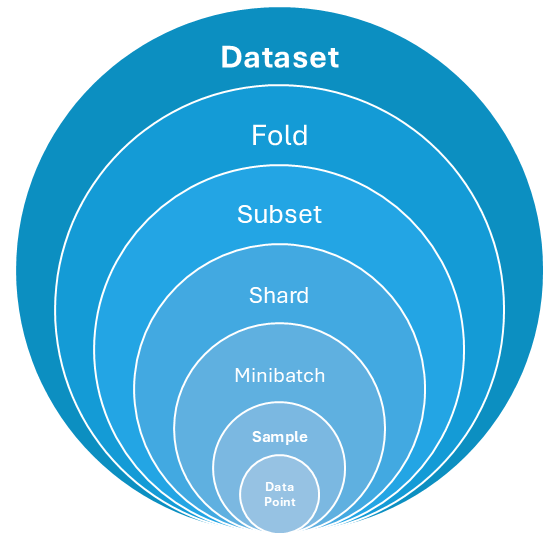
\includegraphics[width=0.4\columnwidth]{fig_datatier/DataTier-Onion.png} 
    \vspace{-0.2in}
    \caption{Depiction of data artifacts as containers of other data artifacts. \label{fig:datatier-onion}}
\end{figure}



The "onion" depiction of data artifacts encapsulates the hierarchical nature of data management within the MANOLO suite. At the core, there are data points, which aggregate into samples. These samples, can belong to mini-batches or shards of multiple mini-batches. The container for those are subsets for training, validation, and testing, which collectively constitute a fold of the dataset for k-Fold cross validation experiments. This layered approach covers any organization of data artifacts, emphasizing the generic approach and scalability of the data tier.

The MANOLO data tier supports a wide range of artifact types, addressing the diverse needs of modern applications. Object/Record Sets represent collections of objects or records with fields that can vary in data type, such as numeric, string, date, or nested objects. Vector Sets consist of fixed-dimensional numeric vectors with uniform data types and ranges, suitable for structured numerical data. Image Sets manage tensors representing grayscale, RGB, or RGB-D images. Point Cloud Sets handle spatial data in three dimensions, where samples are sets of points in a 3D coordinate system. Video Sets accommodate sequences of images over time, capturing dynamic visual data. Time-Series Sets store sensor recordings over time, representing scalar or vector values at discrete timestamps. Graph Datasets encode relationships through vertices and edges, represented in adjacency lists or matrices, with associated values. Spatiotemporal Graph Datasets extend this by incorporating temporal dimensions, allowing each vertex and each edge to have a time series of its values. 

\subsubsection{Experiment artifacts and model registries}
The MANOLO data tier extends its architecture to facilitate the hosting and management of machine learning experiments, encompassing models and associated artifacts. It offers the capability to seamlessly organize and connect various components of an ML experiment, beginning with the model itself and hyperparameters governing its architecture, the data handling and training processes. Each ML experiment is linked to a specific training set from a dataset, ensuring traceability and reproducibility of the training context. The data tier can store the final state of a trained model but also intermediate states during training, also known as checkpoints, including the model parameter state and the training process variable values. These artifacts enable pausing and resuming training sessions or evaluating different stages in a model's training process.

The relational structure of the MANOLO data tier ensures that all these components are interconnected. Models, training sets, and other associated artifacts are represented as objects with unique Object IDs (OIDs), while their relationships are captured using semantic triplets. This approach allows for defining the dependencies and associations between a model, its training data, and the parameters of its training process. Key-value pairs stored in metadata arrays further enrich these objects, providing additional context such as the provenance of the data, hyperparameter configurations, evaluation metrics, and any other relevant details.

The system accommodates various model-related artifacts, each with distinct roles. Model state objects (MS) represent the complete set of parameters and structural definitions for a pre-trained model, enabling efficient storage and retrieval of ready-to-use models. Training state objects (ST) capture the entire set of parameters necessary to resume a paused training session, which may include both the model and additional states related to the training algorithm. Model class objects (MC) define collections of related models, that are either generated during a hyperparameter search, or sharing common characteristics such as common architecture or dataset configurations. Finally, surrogate models (SM) are supported as explainable representations of non-explainable models, providing interpretability while maintaining the original model's predictive capabilities.

Through this architecture, the MANOLO data tier ensures that machine learning experiments are not only efficiently stored but also fully contextualized within a relational framework. By leveraging metadata, semantic relationships, and hierarchical object structures, the system supports complex ML workflows, enabling reproducibility, scalability, and adaptability without delving into the specific implementation details of individual methods.

\subsection{General purpose artifacts}
The data tier in MANOLO is designed to handle a wide variety of file types, accommodating diverse artifacts. These include plain text files such as unstructured text (.TXT) and tabular text formats (.CSV, .XLSX, .ODS), document files, and generic binary files like custom binary formats (.BIN) and compressed binary formats (.ZIP, .TAR). It also supports generic multimedia files, including original and compressed images, raw and encoded video formats. Additionally, the system manages raw and encoded signal data, as well as serialized objects in textual formats (.XML, .JSON) and binary serialized objects (e.g., Pickle, Protobuf). This generic approach allows MANOLO's data tier to handle both structured and unstructured data efficiently across various file types and formats.

\subsubsection{Metadata and semantic relations between artifacts}

Metadata can be attached to artifacts in a flexible way to support various project needs, such as recording metrics after evaluating experiments, or storing series of values from monitoring processes. Each object hosts an associative array to hold metadata in the form of key-value pairs, where the value may contain an objec with multiple fields (e.g., hyperparameter name-value pairs). Metadata can also be structured as a tree, allowing annotations to follow a hierarchical structure. Moreover, they can be organized in any kind of graph, utilizing an adjacency list or matrix for representing complex relationships.

Additionally, semantic triples in the form of subject-predicate-object, are used to define logical relations between artifacts, such as “dataset A is reduced into dataset B” or “model B is an alternative to model A,” providing semantic meaning to the connections between different entities. For tasks requiring relational data, the metadata can be structured as relational rows, where each row corresponds to a set of related values. This flexibility in metadata structure allows MANOLO to support a wide range of tasks, from data reduction and model comparison to more complex monitoring and evaluation processes.

Furthermore, the data tier in MANOLO supports basic querying on these semantic relations, enabling users to easily retrieve useful information to facilitate project tasks. For example, users can query to "list all alternatives of model A" or "list all derived datasets of dataset A," making it easier to explore the relationships between artifacts and enabling more efficient project management and decision-making.

\subsection{Manolo data tier web service}
The MANOLO data tier is a robust and scalable web service built using .NET Core, designed to efficiently handle and store various types of artifacts and metadata. It operates as a \textbf{FastAPI} web service, enabling seamless communication with other systems through standard HTTP methods (GET, POST, PUT, DELETE). This service is deployed within a Docker container, ensuring ease of deployment, scalability, and isolation. It can be deployed on the cloud for shared access or inside the local network edge for isolated use.


The core data management suite of the system is PostgreSQL, an SQL-compatible database that also supports NoSQL features through JSON and JSONB data types. PostgreSQL allows the creation of tables to store structured data, with each data structure (e.g., experiments, models, datasets) having its own dedicated table. For enhanced performance, PostgreSQL is configured with Generalized Inverted Indexes (GIN) to index JSON and JSONB columns, enabling fast and efficient querying of non-relational data. It also supports full-text search capabilities, crucial for querying metadata stored in JSON/JSONB format.
For file storage, MANOLO utilizes the standard Linux file system (ext4) within the Docker container. Files are organized according to the Linux directory structure, ensuring compatibility and ease of access. This system is well-suited for storing large artifacts such as models, datasets, and experiment logs.

Each artifact or metadata entry in MANOLO is associated with a unique identifier, typically a \textbf{Unique Lexicographically Sortable Identifier (ULID)} ensuring global uniqueness across distributed systems. These ULIDs are used to reference and access individual records across the data tier. The system handles a wide range of data types, including structured data (e.g., tabular data, hyperparameters) stored in PostgreSQL tables and unstructured or semi-structured data (e.g., JSON/JSONB, raw files) stored in both PostgreSQL and NoSQL databases. Object of large volume, like model states or large-scale datasets, can also be stored in an auxiliary tensor store database to leverage high-performance operations and efficient storage schemes.

In the MANOLO system, each artifact type has a specific table in the database. For every data structure entry, a corresponding table named Items is created within the PostgreSQL database. Each record in the table contains a unique identifier implemented using ULIDs, a data field capable of storing variable-sized content in byte format, a field that specifies the type of data stored, and a timestamp that tracks the last modification of the entry. This design provides a generic approach to storing any artifact within the MANOLO framework.

The MANOLO data tier employs robust security measures to safeguard the confidentiality, integrity, and proper access control of artifacts. User authentication is managed through cookie-based authentication, which is mandatory for accessing or interacting with system endpoints. Each endpoint is governed by a designated authorization policy, with access determined by the cookie issued to the user during the sign-in process. This mechanism allows for the definition of access attribute flags tailored to each endpoint's requirements.

The system currently supports three authentication policies:
\begin{itemize}
    \setlength{\itemsep}{0pt}
    \setlength{\parskip}{0pt}
    \item \textbf{All}, which grants access to endpoints open to all users;
    \item \textbf{ModeratorOrHigher}, which permits access to most endpoints; and
    \item \textbf{AdminOnly}, which provides access to all endpoints.
\end{itemize}

These access logs allow for detailed tracking and auditing of user activity, helping detect unauthorized access and ensure compliance with security policies.

For data protection, MANOLO supports both encryption during transfer and storage. Data in transit is protected using transport layer encryption, such as TLS 1.3, to ensure confidentiality and integrity while being transmitted. For storage encryption, artifact objects that are not actively queried or are infrequently accessed could be encrypted when stored using symmetric end-to-end encryption, such as AES-256. Importantly, the symmetric encryption uses the end user to manage their encryption key, ensuring they maintain full control over access to sensitive data. This encryption process ensures that only authorized users with the correct decryption keys can access sensitive artifact content. Overall, the combination of authentication, access control, access logging, and encryption provides a strong security framework to safeguard data throughout the lifecycle of the project.

\subsection{Data tier web API reference}
The Data Tier Web API Reference provides an overview of the key endpoints used for managing data within the system. It covers operations for creating, retrieving, updating, deleting and restoring various entities such as data structures, items, predicates, relations, aliases and key-value pairs. Additionally, it includes authentication and management functionalities, such as user login and database backup and restore. Each section outlines available endpoints, their purpose, and the parameters required, offering a clear and concise framework for interacting with the API. This reference is designed to help efficiently utilize the system’s capabilities while ensuring consistency and reliability in data management.


\subsubsection{Data Structures}
%=================================================================================================
\begin{longtable}
    \centering
    \renewcommand{\arraystretch}{1.2}
    \begin{tabular}{|p{0.25\linewidth}|p{0.75\linewidth}|}
% -----------------------------------------------------------------------
\hline
    \underline{Method Name} & \underline{Description} 
\\
% -----------------------------------------------------------------------    
\hline \textbf{GetDataStructures} & Summary: Handles the request to retrieve a list of data structures from the database.

Returns: A Result object containing a list of data structure IDs if any exist, or a failure result with a domain error if no data structures are found.
\\       
% ----------------------------------------------------------------------- 
\hline \textbf{CreateDataStructure} & Summary: Handles the creation of a new data structure.

Parameters:

- Request: The CreateDataStructureQuery containing the details of the data structure to be created.

Returns: A Task that represents the asynchronous operation. The task result contains a Result object. If successful, the Result contains the ID of the newly created data structure. If a data structure with the same name or DSN already exists, the Result indicates a failure with an appropriate error message.
\\     
% -----------------------------------------------------------------------
\hline \textbf{DeleteDataStructure} & Summary: Handles the deletion of a DataStructure based on the provided request.

Parameters:

- Request: The request containing the DataStructures ID, DSN, or Name to be deleted.

Returns: A Result object indicating the success or failure of the deletion operation, along with any relevant error messages.
\\
% -----------------------------------------------------------------------
\hline \textbf{GetDataStructure} & Summary: Summary: Handles the request to get a specific data structure by its ID.

Parameters:

- Request: The request containing the ID of the data structure to retrieve.

Returns: A Result object containing the retrieved data structure if it exists, or a failure result with a domain error if the data structure does not exist.
\\
% -----------------------------------------------------------------------
\hline \textbf{RestoreDataStructure} & Summary: Handles the request to restore a data structure.

Parameters:

- Request: The request containing the data structures ID, DSN, or name to be restored.

Returns: A Result object indicating the success or failure of the restore operation, along with a message.
\\
% -----------------------------------------------------------------------
\hline \textbf{UpdateDataStructure} & Summary: Handles the update of a data structure.

Parameters:

- Request: The request containing the data structures id and updated properties.

Returns: A Result object indicating the success or failure of the operation, along with any relevant error messages.
\\
% ----------------------------------------------------------------------- 

        \hline
    \end{tabular}
\end{longtable}
%=================================================================================================





\newpage
\subsubsection{Items}
%=================================================================================================
\begin{longtable}
    \centering
    \renewcommand{\arraystretch}{1.2}
    \begin{tabular}{|p{0.25\linewidth}|p{0.75\linewidth}|}
% -----------------------------------------------------------------------     
\hline
    \underline{Method Name} & \underline{Description} 
\\
% ----------------------------------------------------------------------- 
\hline
    \textbf{CreateItem} & Summary: Handles the creation of a new item based on the provided request.
    
Parameters:

- Request: The create item query containing the necessary data for item creation.

Returns: A task that represents the asynchronous operation. The result of the task is a Result object indicating success or failure, along with the new items ID.
\\
% ----------------------------------------------------------------------- 
\hline
    \textbf{DeleteItem} & Summary: Handles the deletion of an item based on the provided request.
    
Parameters:

- Request: The delete item query containing the DSN and item ID.

Returns: A Result indicating the success or failure of the deletion operation.
\\
% ----------------------------------------------------------------------- 
\hline
    \textbf{DownloadItemData} & Summary: Handles the download of item data based on the provided DSN and item ID.
    
Parameters:

- Request: The download item data query containing the DSN and item ID.

Returns: An IActionResult representing the downloaded file or a NotFoundResult if the item or data structures are not found.
\\
% ----------------------------------------------------------------------- 
\hline
    \textbf{GetItem} & Summary: Handles the GetItemQuery request by retrieving an item from the database based on the provided DSN and item ID.
    
Parameters:

- Request: The GetItemQuery request containing the DSN and item ID.

Returns: A Result object containing the retrieved item if successful, or an error message if the item does not exist or an error occurs.
\\
% ----------------------------------------------------------------------- 
\hline
    \textbf{GetItemData} & Summary: Handles the GetItemDataQuery request to retrieve item data based on the provided DSN and item ID.
    
Parameters:

- Request: The GetItemDataQuery request containing the DSN and item ID.

Returns: A Result object indicating the success or failure of the operation. If successful, the Result contains the decoded item data as a string. If unsuccessful, the Result contains a DomainError indicating the specific error.
\\
% ----------------------------------------------------------------------- 
\hline
    \textbf{GetItems} & Summary: Handles the GetItemsQuery request to retrieve a list of items based on the provided DSN.
    
Parameters:

- Request: The GetItemsQuery request containing the DSN.

Returns: A Result object indicating the success or failure of the operation. If successful, the Result contains a list of item IDs. If unsuccessful, the Result contains a DomainError indicating the reason for the failure.
\\
% ----------------------------------------------------------------------- 
\hline
    \textbf{RestoreItem} & Summary: Handles the restore operation for a specific item in the database.
    
Parameters:

- Request: The restore item query containing the DSN and item ID.

Returns: A Result indicating the success or failure of the restore operation.
\\
% ----------------------------------------------------------------------- 
\hline
    \textbf{UpdateItem} & Summary: Handles the update of an item in the database.

Parameters:

- Request: The update item query containing the necessary parameters.

Returns: A Result indicating the success or failure of the operation.
\\
% ----------------------------------------------------------------------- 
        \hline
    \end{tabular}
\end{longtable}
       
%=================================================================================================


\newpage
\subsubsection{Predicates}
%=================================================================================================
\begin{longtable}
    \centering
    \renewcommand{\arraystretch}{1.2}
    \begin{tabular}{|p{0.25\linewidth}|p{0.75\linewidth}|}
% -----------------------------------------------------------------------    
\hline
    \underline{Method Name} & \underline{Description} 
\\
% -----------------------------------------------------------------------
\hline
    \textbf{CreatePredicate} & Summary: Handles the creation of a new predicate.
    
Parameters:

- Request: The request containing the description of the predicate to be created.

Returns: A Result representing the asynchronous operation. The task result contains the unique identifier of the newly created predicate if successful, or an error message if the predicate already exists.
\\
% -----------------------------------------------------------------------
\hline
    \textbf{DeletePredicate} & Summary: Handles the deletion of a predicate based on the provided description.
    
Parameters:

- Request: The delete predicate query contains the description of the predicate to be deleted.

Returns: A task that represents the asynchronous operation. 	The task result is a Result indicating the success or failure of the operation. If the predicate with the given description does not exist, the result will be a failure with a corresponding error.
\\
% -----------------------------------------------------------------------
\hline
    \textbf{GetObjectsOfPredicate} & Summary: Handles the request to get objects related to a specific predicate.
    
Parameters:
- Request: The request containing the predicate description.

Returns: A Result object indicating success or failure. If successful, the Result contains a list of objects related to the predicate. If unsuccessful, the Result contains a DomainError indicating the reason for failure.
\\
% -----------------------------------------------------------------------
\hline
    \textbf{GetPredicates} & Summary: Handles the GetPredicatesQuery request to retrieve a list of predicates from the database.
   
Parameters:

- Request: The GetPredicatesQuery request object containing any necessary parameters.

Returns: A Result object indicating the success or failure of the operation. If successful, the Result contains a list of existing predicates. If unsuccessful, the Result contains a DomainError indicating the reason for the failure.
\\
% ----------------------------------------------------------------------- 
\hline
    \textbf{GetSubjectsOfPredicate} & Summary: Handles the request to retrieve subjects related to a specific predicate.
    
Parameters:

- Request: The request containing the predicate description.

Returns: A Result representing the asynchronous operation. The result contains either a list of subjects related to the predicate or an error message.
\\
% ----------------------------------------------------------------------- 
\hline
    \textbf{GetSubjectsOf} & Summary: Handles the GetSubjectsOfQuery request to retrieve the subjects related to a specific object.
    
Parameters:

- Request: The GetSubjectsOfQuery request containing the object and predicate description.

Returns: A Result object indicating the success or failure of the operation. 	If successful, the Result contains a list of related subjects. If unsuccessful, the Result contains a DomainError indicating the reason for the failure.
\\
% ----------------------------------------------------------------------- 
\hline
    \textbf{GetObjectsOf} & Summary: Handles the GetObjectsOfQuery request to retrieve objects related to a given subject.
    
Parameters:

- Request: The GetObjectsOfQuery request containing the subject and description.

Returns: A Result object indicating success or failure. If successful, the Result contains a list of related objects. If failure, the Result contains a DomainError indicating the reason for the failure.
\\
% ----------------------------------------------------------------------- 
        \hline
    \end{tabular}
\end{longtable}        
%=================================================================================================


\newpage
\subsubsection{Relations}
%=================================================================================================
\begin{longtable}
    \centering
    \renewcommand{\arraystretch}{1.2}
    \begin{tabular}{|p{0.25\linewidth}|p{0.75\linewidth}|}
% -----------------------------------------------------------------------     
\hline
    \underline{Method Name} & \underline{Description} 
\\
% ----------------------------------------------------------------------- 
\hline
    \textbf{CreateRelation} & Summary: Handles the creation of a new relation between two entities (subject and object) based on the given predicate and 	DSN.
    
Parameters:

- Request: The create relation query containing the necessary parameters.

Returns: A task that represents the asynchronous operation. 	The result is an indication of success or failure. If successful, the result is Result.Success; otherwise, it is Result.Failure with an appropriate error.
\\
% ----------------------------------------------------------------------- 
\hline
    \textbf{DeleteRelation} & Summary: Handles the deletion of a relation between two entities in the ManoloDataTier system.
    
Parameters:

- Request: The delete relation query containing the details of the relation to be deleted.

Returns: A Result indicating the success or failure of the deletion operation.
\\
% ----------------------------------------------------------------------- 
\hline
    \textbf{GetRelations} & Summary: Handles the GetRelationsQuery request to retrieve a list of relations from the database.
    
Parameters:

- Request: The GetRelationsQuery request containing any necessary parameters.

Returns: A Result object containing either a list of relations or an error message. If the list of relations is empty, it returns a failure Result with a NoRelations domain error. Otherwise, it returns a success Result with the list of relations.
\\
% ----------------------------------------------------------------------- 
\hline
    \textbf{AddChild} & Adds a child item object under a parent item object in a tree data structure.
    
Parameters:

- DSN: data structure number.

- Parent: parent object ID

- Child: child object ID
\\
% ----------------------------------------------------------------------- 
\hline
    \textbf{GetChildren} & Return a list with the object IDs for the children of the given parent item in a tree data structure.
    
Parameters:

- DSN: data structure number.

- Parent: parent object ID
\\
% ----------------------------------------------------------------------- 
\hline
    \textbf{AddEdge} & Add an edge between two node item objects in a graph data structure.
    
Parameters:

- DSN: data structure number.

- node1:  first (source) node object ID

- node2:  second (destination) node object ID

- value (optional):  the value for the edge

- is\textunderscore directed (optional): | 0 (default) undirected edge | 1: directed edge. 
\\
% ----------------------------------------------------------------------- 
\hline
    \textbf{GetAdjacencyList} & Return a list with the object IDs for the adjacent nodes to the given node item in a graph data structure.
    
Parameters:

- DSN: data structure number.

- node: node object ID.
\\
% ----------------------------------------------------------------------- 
        \hline
    \end{tabular}
\end{longtable}       
%=================================================================================================



\newpage
\subsubsection{Global Aliases}
%=================================================================================================
\begin{longtable}{c}
    \renewcommand{\arraystretch}{1.2}
    \begin{tabular}{|p{0.25\linewidth}|p{0.75\linewidth}|}
% -----------------------------------------------------------------------     
\hline
    \underline{Method Name} & \underline{Description} 
\\
% ----------------------------------------------------------------------- 
\hline
    \textbf{CreateUpdateAlias} & Summary: Handles the creation or update of an alias.
    
Parameters:

- Request: The CreateUpdateAliasQuery containing the alias details to be created or updated.

Returns: A Task that represents the asynchronous operation, containing a Result object. The Result is successful if the alias was created or updated, or a failure if an alias with the same name already exists.
\\
% ----------------------------------------------------------------------- 
\hline
    \textbf{DeleteAlias} & Summary: Handles the deletion of an alias based on the provided query.
    
Parameters:

- Request: The DeleteAliasQuery containing the alias name to be deleted.

Returns: A Result object indicating the outcome of the deletion operation. It would be a Success result if the alias was successfully deleted, or a Failure result with an AliasDoesNotExist error if no alias was found.
\\
% ----------------------------------------------------------------------- 
\hline
    \textbf{GetAlias} & Summary: Handles the GetAliasQuery request by retrieving an alias from the database.

Parameters:

- Request: The GetAliasQuery containing the ID of the alias to retrieve.

Returns: A Result object containing: 	

- Success with the alias name if the alias is found. 	

- Failure with a DomainError if the alias is not found.
\\
% ----------------------------------------------------------------------- 
\hline
    \textbf{GetId} & Summary: Handles the GetIdQuery request by retrieving the ID of an alias from the database.
    
Parameters:

- Request: The GetIdQuery object containing the alias name to search for.

Returns: A Result object containing either: 	- A successful result with the ID of the found alias, or 	- A failure results in an AliasDoesNotExist error if the alias is not found.
\\
% ----------------------------------------------------------------------- 
        \hline
    \end{tabular}
\end{longtable}      
%=================================================================================================



\newpage
\subsubsection{Key-Value Pairs}
%=================================================================================================
\begin{longtable}{c}
    \renewcommand{\arraystretch}{1.2}
    \begin{tabular}{|p{0.25\linewidth}|p{0.75\linewidth}|}
% -----------------------------------------------------------------------     
\hline
    \underline{Method Name} & \underline{Description} 
\\
% ----------------------------------------------------------------------- 
\hline
    \textbf{CreateUpdateKeyValue} & Summary: Handles the creation or update of a Key-Value pair in the database.

Parameters:

- Request: The request containing the Key-Value data.

Returns: A Result indicating the success or failure of the operation.
\\
% ----------------------------------------------------------------------- 
\hline
    \textbf{DeleteKeyValue} & Summary: Handles the deletion of a key-value pair from the database.
    
Parameters:

- Request: The delete key-value query containing the key to be deleted.

Returns: A Result representing the asynchronous operation. The result is an indication of success or failure. If the key does not exist in the database, the result will be a failure with a corresponding error.
\\
% ----------------------------------------------------------------------- 
\hline
    \textbf{GetKeys} & Summary: Handles the GetKeysQuery request to retrieve all keys associated with a specific object.
    
Parameters:

- Request: The GetKeysQuery request containing the object for which keys are requested.

Returns: A Result object indicating the success or failure of the operation. If successful, the Result contains a list of keys associated with the object. If unsuccessful, the Result contains a DomainError indicating the reason for the failure.
\\
% ----------------------------------------------------------------------- 
\hline
    \textbf{GetValue} & Summary: Handles the logic for retrieving a value associated with a given key from the database.
    
Parameters:

- Request: The request containing the key to retrieve.

Returns: A Result representing the asynchronous operation. The result is a Result object containing the retrieved value if the key exists, or an error message if the key does not exist.
\\
% ----------------------------------------------------------------------- 
        \hline
    \end{tabular}
\end{longtable}     
%=================================================================================================



\subsubsection{Authentication}
%=================================================================================================
\begin{longtable}{c}
    \renewcommand{\arraystretch}{1.2}
    \begin{tabular}{|p{0.25\linewidth}|p{0.75\linewidth}|}
% -----------------------------------------------------------------------     
\hline
    \underline{Method Name} & \underline{Description} 
\\
% ----------------------------------------------------------------------- 
\hline
    \textbf{AddUser} & Summary: Handles the addition of a new user to the database.
    
Parameters:

- Request: The AddUserQuery containing the new user's information.

Returns: A Task that represents the asynchronous operation, containing a Result object. The Result is successful if the user was added, or a failure with an error message if the username already exists.
\\
% ----------------------------------------------------------------------- 
\hline
    \textbf{Login} & Summary: Handles the login process for a user.
    
Parameters:

- Request: The login query containing the username and password.

Returns: A Result object indicating the outcome of the login attempt. Returns a success result if the login is successful, or a failure result if the user does not exist or the password is  incorrect.
\\
% ----------------------------------------------------------------------- 
\hline
    \textbf{Logout} & Summary: Handles the logout process for the current user.
    
Returns: A Result object indicating the success of the logout operation.
\\
% ----------------------------------------------------------------------- 
        \hline
    \end{tabular}
\end{longtable}       
%=================================================================================================



\newpage
\subsubsection{Management}
%=================================================================================================
\begin{longtable}{c}
    \renewcommand{\arraystretch}{1.2}
    \begin{tabular}{|p{0.25\linewidth}|p{0.75\linewidth}|}
% -----------------------------------------------------------------------     
\hline
    \underline{Method Name} & \underline{Description} 
\\
% ----------------------------------------------------------------------- 
\hline
    \textbf{Backup} & Summary: Handles the backup request by retrieving data from the database and storing it in a JSON file.
    
Returns: A Result indicating the success or failure of the backup operation.
\\
% ----------------------------------------------------------------------- 
\hline
    \textbf{Restore} & Summary: Handles the restore operation by processing the backup data and restoring it to the database.
    
Parameters:

- Request: The restore query containing the backup data.

Returns: A task that represents the asynchronous operation. The result is an indication of success or failure.
\\
% ----------------------------------------------------------------------- 
        \hline
    \end{tabular}
\end{longtable}    
%=================================================================================================